%%%% TODO

%%%%%%%%%%%%%%%%%%%%%%%%%%%%%%%%%%%%%%%
%%% LATEX HEADERS
%%%%%%%%%%%%%%%%%%%%%%%%%%%%%%%%%%%%%%%

\documentclass[article]{JSSstyle/jss}
\usepackage{rotating}                           
\usepackage[dvips]{epsfig}
\usepackage{multirow}
\usepackage{amsfonts,amssymb,amsmath}
\usepackage{array}                      
\usepackage{url}
\usepackage{thumbpdf}
\usepackage{natbib}

\usepackage{vmargin}
    \setpapersize{USletter}
    \setmarginsrb{1.0in}{1.0in}{1.0in}{1.0in}{0.5in}{0.2in}{0in}{0.2in}
\renewcommand{\baselinestretch}{1.25}

%%%%%%%%%%%%%%%%%%%%%%%%%%%%%%%%%%%%%%%
%%% SHORTCUTS
%%%%%%%%%%%%%%%%%%%%%%%%%%%%%%%%%%%%%%%

% open office tricks
\newcommand\textsubscript[1]{\ensuremath{{}_{\text{#1}}}}

%%%%%%%
%%% Vignette Headers
%%%%%%%

%\VignetteIndexEntry{bard}
%\VignetteKeywords{automated redistricting}
%\VignetteVersion{1.0}
%\VignetteTitle{Better Automated redistricting} 

%%%%%%%%%%%%%%%%%%%%%%%%%%%%%%%%%%%%%%%
%%% DOCUMENT HEADERS
%%%%%%%%%%%%%%%%%%%%%%%%%%%%%%%%%%%%%%%

\author{Micah Altman\\Harvard University
\And Michael P. McDonald \\George Mason University\\Brookings Institution
}
\Plainauthor{Micah Altman, Michael P. McDonald}
\title{\pkg{BARD}: Better Automated Redistricting}
\Plaintitle{BARD: Better Automated Redistricting}
\Shorttitle{\pkg{Better Automated Redistricting}}
\Keywords{redistricting, optimization}

\Address{
Micah Altman\\
Senior Research Scientist\\
Institute for Quantitative Social Science\\
Harvard University\\
1737 Cambridge Street, N325\\ 
Cambridge, MA, 02138.\\
United States of America\\
E-mail: \email{micah\_altman@harvard.edu}\\
URL: \url{http://maltman.hmdc.harvard.edu/}\\
\\
Michael P. McDonald\\
Associate Professor, Department of Public and International Affairs\\
George Mason University\\
4400 University Drive - 3F4\\
Fairfax, VA 22030-4444 \\
E-mail: \email{mmcdon@gmu.edu}\\
URL: \url{http://elections.gmu.edu/}\\
}

\Abstract{
\pkg{BARD} is the first (and at time of writing, only) open source software package for general redistricting and redistricting analysis. \pkg{BARD} provides methods to create, display, compare, edit, automatically refine, evaluate, and profile political districting plans.  \pkg{BARD} aims to provide a framework for scientific analysis of redistricting plans and to facilitate wider public participation in the creation of new plans.

\pkg{BARD} facilitates map creation and refinement through command-line, gui, and automatic methods. Since redistricting is a computationally complex partitioning problem not amenable to 
an exact optimization solution, \pkg{BARD} implements a variety of selectable metaheuristics that can be used to refine existing or randomly-generated redistricting plans based on user-determined criteria. 

Furthermore, \pkg{BARD} supports automated generation of redistricting plans and profiling of plans by assigning different weights to various criteria, such as district compactness or equality of population. This functionality permits exploration of trade-offs among criteria. The intent of a redistricting authority may be explored by examining these trade-offs and inferring which reasonably observable plans were not adopted.

Redistricting is a computationally-intensive problem for even modest-sized states. Performance is thus an important consideration in \pkg{BARD}'s design and implementation. The program implements performance enhancements such as evaluation caching, explicit memory management, and distributed computing across \pkg{snow} clusters.
}

%%% Below is a magic header line, with two %:
%% need no \usepackage{Sweave.sty}



%%%%%%%%%%%%%%%%%%%%%%%%%%%%%%%%%%%%%%%
%%% DOCUMENT STARTS
%%%%%%%%%%%%%%%%%%%%%%%%%%%%%%%%%%%%%%%

\begin{document}

\section{Introduction}

Legislative redistricting is among the most politically charged 
tasks in American politics.  District lines affect which political 
party wins control of a legislative body, the reelection success of 
incumbents, and election of minority preferred candidates. 

In the 1960s, after the U.S. Supreme Court's landmark decisions requiring equal population in districts, scholars envisioned taking politics out of redistricting by 
programming computers to automatically draw districts \citep[][]{Vickrey61,WeaverHess63,Nagel1965}. These scholars reasoned that an algorithm implementing 
politics-blind criteria would draw districts neutral to politics. 

Automated redistricting programs were developed, and special purpose software was developed (and even freely distributed \citep[see]{Nagel1965}) for this purpose,  but the problem was too computationally difficult to solve practically.  Instead, computers were found to be well-suited to assist human planners in processing the large amounts of population, election, and geo-spatial  redistricting data.  And it was out of this use that some of the first Geographic Information Systems (GIS) 
were born \citep{AltMacMcD05}.  

Unfortunately, early computerized redistricting systems were prohibitively expensive to all but state governments or political parties, effectively shutting out the public from the redistricting process. Computer hardware and specialized redistricting GIS software have since become more affordable. However, specialized software packages for redistricting still remain unusually expensive -- costing thousands of dollars. We aim to make the redistricting process more open, by  offering the first open-source general redistricting software. We call our computer program \pkg{BARD} for \textbf{B}etter \textbf{A}utomated 
\textbf{R}e\textbf{D}istricting.\footnote{Tolkein fans may recognize the 
reference to the slayer of the dragon Smaug, perhaps the most 
terrible of salamanders.}

Our package permits users to draw and compare redistricting `plans'.\footnote{A plan consists of a geographic map of some administrative unit, such as census tracts or counties, along with political and demographic measurements for each unit, and an assignment of those units to a set of districts.} Our package also permits users to evaluate whether these meet legal requirements, and measure their potential political consequences. The system is open and extendable, so that anyone can a wide variety of built-in measures, or add any they desire, to evaluate plans.  \pkg{BARD}  is not only the first  \emph{open source} package for general redistricting analysis, it is also the first publicly available redistricting package to support multi-criteria optimization for redistricting plans.

\section[Redistricting with BARD]{Redistricting with \pkg{BARD}}

Currently \pkg{BARD} provides functionality in multiple areas, and the implementation of the \pkg{BARD} system is divided into separate independent modules to facilitate maintenance and flexibility.

\begin{figure}[!h]
The figure below illustrates these areas, and the typical phases of redistricting in \pkg{BARD} 

  \begin{center}
    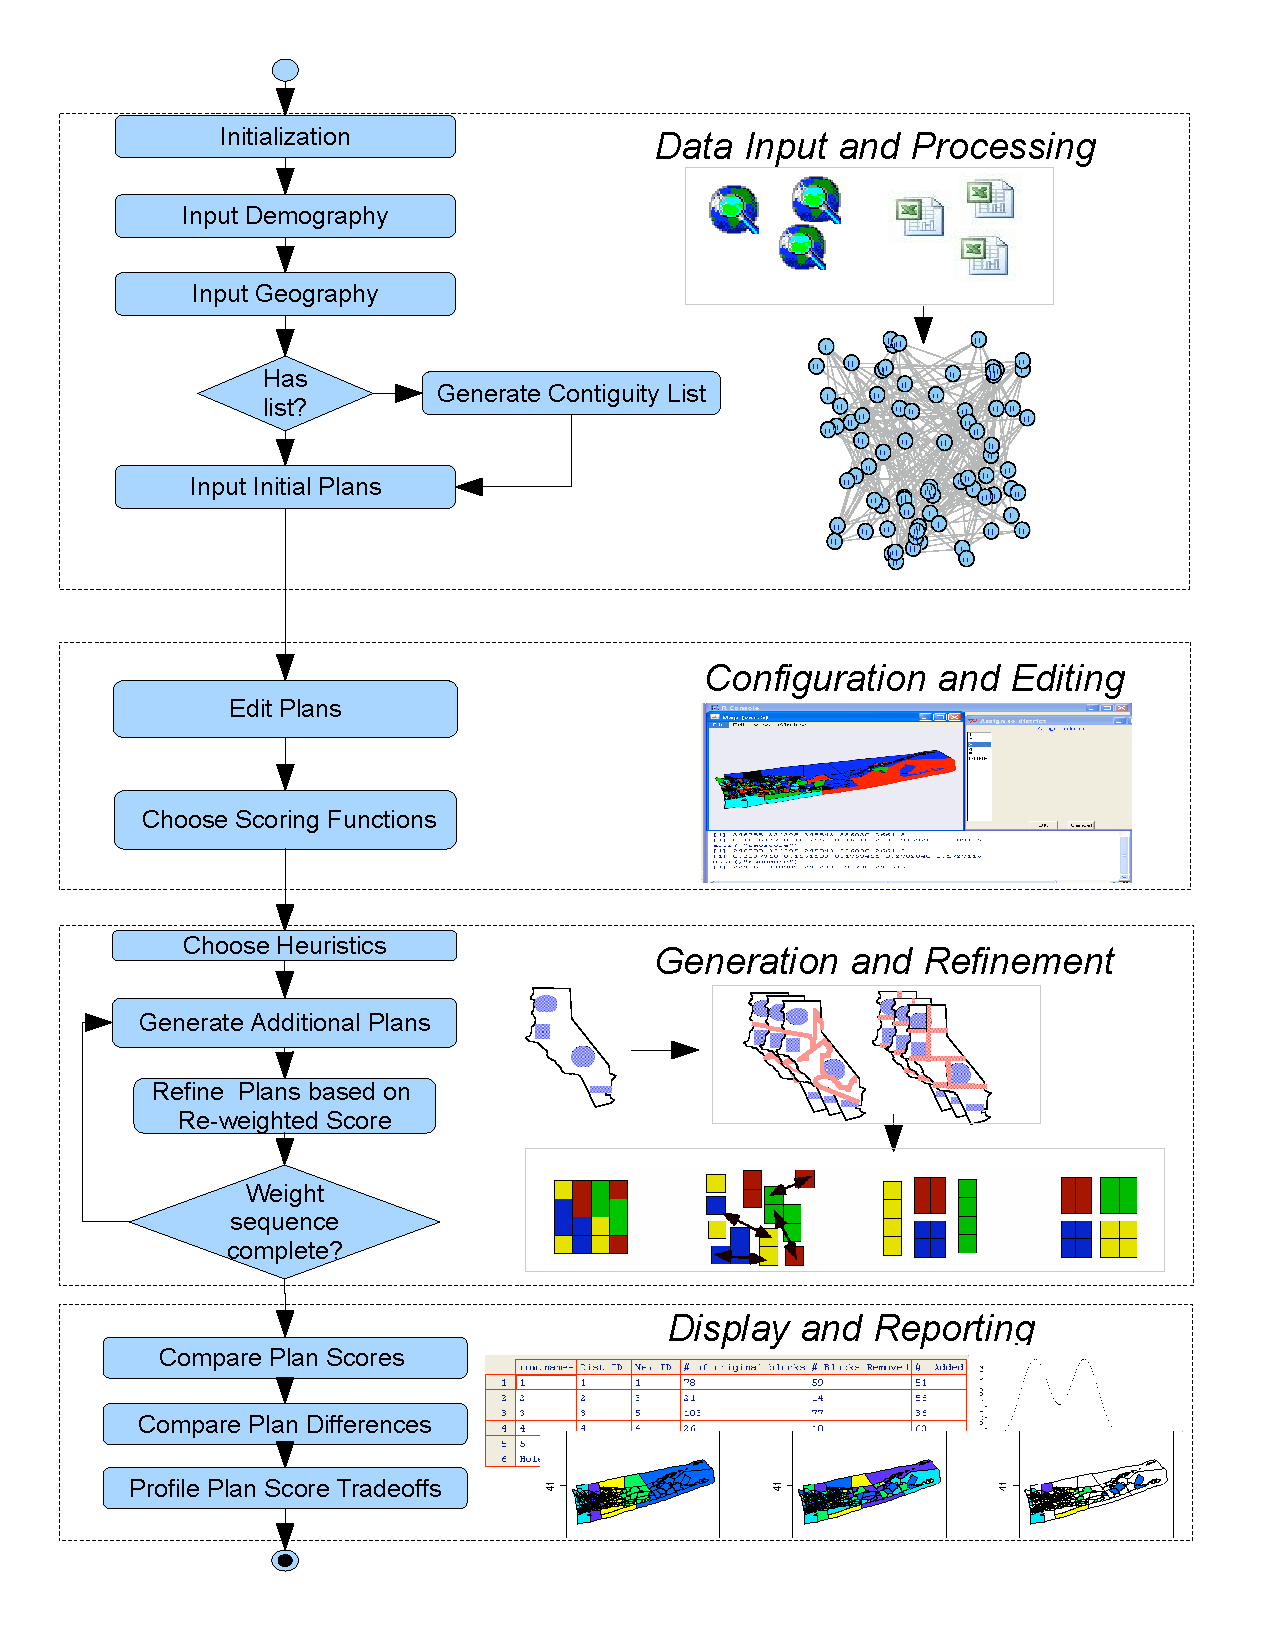
\includegraphics[page=1]{bardiagram.pdf}
  \end{center}

  \caption{\small Phases of redistricting in BARD.}
  \label{fig:barddiagram}
\end{figure}

First, \pkg{BARD} reads and processes redistricting data. \pkg{BARD} can read and write files representing redistricting plans in the standard ESRI ``shapefile'' format, permitting inter-operability with other GIS packages. Inter-operability is desirable since, while \pkg{BARD} has some rudimentary functionality for basic interactive map drawing, existing commercial GIS software has more sophisticated manual map-drawing tools and GUI interfaces. Furthermore, we hope that a redistricting authority will consider a plan drawn with the aid of \pkg{BARD}, which necessarily requires map export functionality. Like these other GIS programs, additional demographic and political data can be imported into \pkg{BARD} that may be essential to evaluate and optimize redistricting plans on.\footnote{At this stage \pkg{BARD} also generates a contiguity analysis of maps in preparation for later manipulation.}

Second, \pkg{BARD} evaluates redistricting plans. \pkg{BARD} will generate textual and graphical reports for a single plan or comparision of multiple plans. Currently \pkg{BARD}  shows precinct-level differences between pairs of plans, counts `holes' in plans, computes common compactness scores, calculates overall population deviation, and checks for contiguity. \pkg{BARD} computes many common political measures, such as number of majority-minority districts, plan competitiveness, etc. Since \pkg{BARD} is built on \proglang{R}, evaluation is extensible to any scoring method that can be programmed into \proglang{R}.

Third, \pkg{BARD} \emph{generates} and \emph{refines} districting plans. Plans can be automatically generated to use as starting points in further refinement, or evaluated in their own right. A user may also choose to start refinement from pre-existing plans (e.g. chosen by the legislature, or offered by a public interest group), if available. We provide a number of different procedures for automatically generating plans including plans for pure random generation of districts (e.g., as described in \citet{Grofman82}), random-walk based methods for generating contiguous equi-populous districts, including methods described in \citet{CirDarOro00}, and both simple and weighted \emph{k}-means based plan generation. Once generated (or provided), plans may be automatically refined using metaheuristics discussed below to meet chosen goals. The application of a metaheuristic to refine plans should yield a plan that is an improvement, given a chosen scoring formula.  

The third phase may vary in some important ways, depending on a user's intended use of the program. For pure applied redistricting, the generation step is omitted and refinement is used to improve existing redistricting plans. For `random' redistricting analysis, such as to probe the characteristics of arbitrary redistricting plans (see \citet{EngWild77,RosJohn81,Oloughlin82,Grofman82} and \citet{CirDarOro00}), generation may be used without refinement, or with refinement only to absolute legal requirements. Analysis of legal constraints on redistricting, as in \citet{Altman97} and \citet{RogersonYang99}, may involve repeated generation and refinement. \pkg{BARD} further supports automated re-weighting of a score function to generate a profile of how one redistricting criterion changes as another is optimized and in this manner \pkg{BARD} will automatically generate profiles of plans that explore tradeoffs among redistricting criteria. (This is computationally expensive, thus \pkg{BARD} supports distributing these calculations across a computing cluster.)

Fourth, \pkg{BARD} compares multiple plans.  \pkg{BARD} outputs the range of overall scores, the range of scores for each component, the differences among plans, and the correlations among score components. Candidate plans may also be contrasted with the starting plans if meaningful pre-existing starting points are selected. This analysis phase can be used to probe redistricting trade-offs -- to what extent attempting to improve plans based on one criterion necessarily reduces performance on other criteria.

\section[Example: Using BARD for Plan Evaluation and Modification]{Using \pkg{BARD} for Plan Evaluation and Modification}

This section demonstrates some of the basic redistricting functions in \pkg{BARD}. These functions permit users to load existing plans into \pkg{BARD} or instruct 
the program to automatically generate a quasi-random map, permit users to manually edit plans, 
and report plan comparisons. In the next section we introduce the mathematical basis for these functions 
and the more complex metaheuristics used to optimize redistricting plans.  

This command loads the \pkg{BARD} package:

\begin{Schunk}
\begin{Sinput}
> library(BARD)
\end{Sinput}
\end{Schunk}

This command imports a standard ``shapefile'' into \pkg{BARD} which will be used as the base map.
The file contains the coordinates of the outlines of all geographical units (the smallest of which in the United States context are known as `census blocks') along with any political and demographic variables in each unit. Our example dataset describes Suffolk County, New York. Optionally, a user can supply a variable in this file that indicates the district to which each unit is currently assigned, thereby enabling evaluation of existing plans. 

\begin{Schunk}
\begin{Sinput}
> suffolk.map <- importBardShape(file.path(system.file("shapefiles", 
+     package = "BARD"), "suffolk_tracts"))
\end{Sinput}
\end{Schunk}

These commands illustrate are several \pkg{BARD} functions that create ``random'' redistricting plans:
\begin{itemize}
	\item \code{createRandomPlan}: Uses pure random assignment.
	\item \code{createRandomPopPlan}: Uses pure random assignment until a district reaches a target population threshold.
	\item \code{createKmeansPlan}: Uses kmeans on geographical district centroids.
	\item \code{createWeightedKmeansPlan}: Weights kmeans by a variable, such as population.
	\item \code{createContiguousPlan}: Attempts to create contiguous plans through the random-walk method of \citet{CirDarOro00}.
\end{itemize}
More information on these functions is included in the documentation accompanying the package.

Two of these functions are illustrated below:
\begin{Schunk}
\begin{Sinput}
> kplan <- createKmeansPlan(suffolk.map, 5)
> rplan <- createRandomPlan(suffolk.map, 5)
\end{Sinput}
\end{Schunk}

The results of these are preliminary assignments of geographic units to districts -- the assignments will need to be refined extensively in most cases to yield a legal plan. 

\pkg{BARD} supports simple plotting of plans as well:

  \begin{figure}[!h]
\begin{Schunk}
\begin{Sinput}
> plot(kplan, cols = colorRampPalette(c("red", "grey"))(5), axes = F)
\end{Sinput}
\end{Schunk}
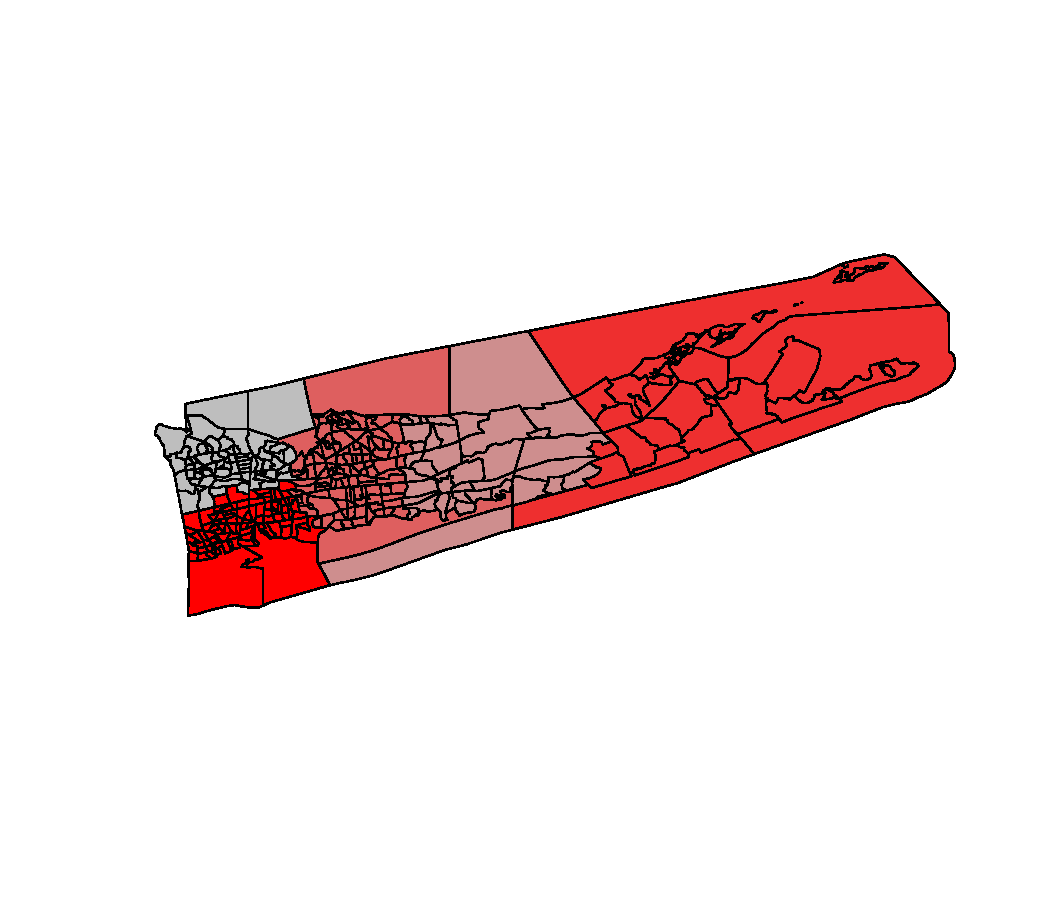
\includegraphics{bardJSS-plot1a}
  \caption{\label{fig:rplot1} Plotting a sample plan}
  \end{figure}

  % WORKAROUND LATEX FIGURE LOCATION prob
\newpage
In addition to plan generation, \pkg{BARD} supports basic interactive editing of plans (here, by reassigning census blocks among districts).

\begin{figure}[!h]
  The interactive map generation interface is illustrated below:
  \begin{center}
    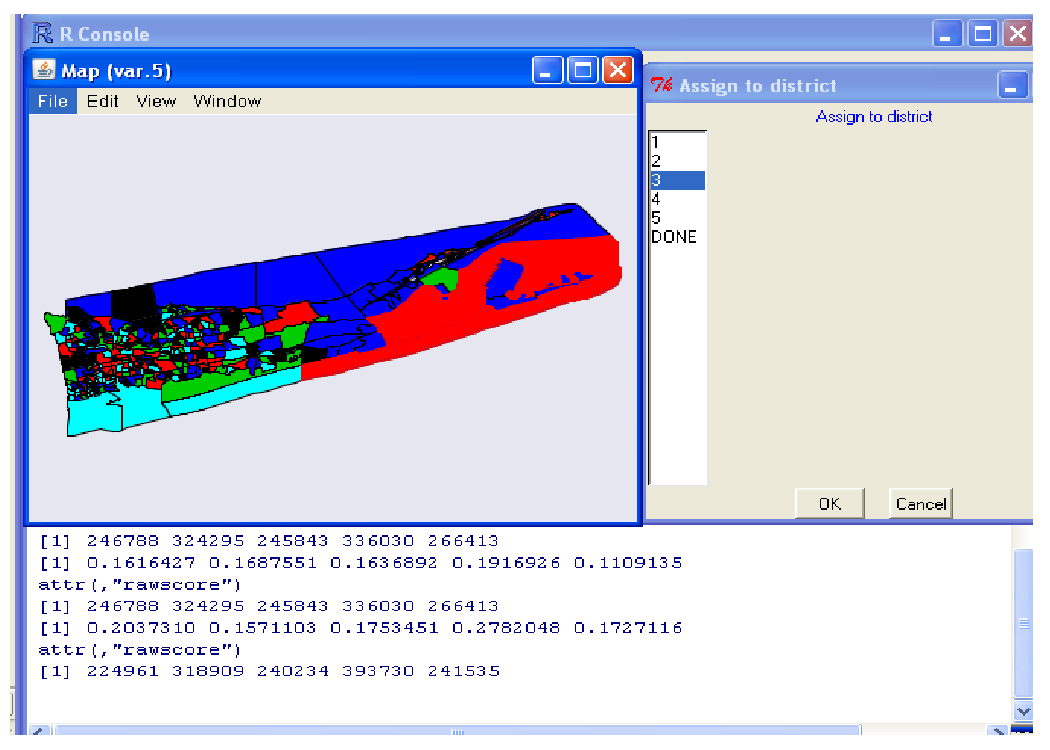
\includegraphics[page=1]{edit_map.pdf}
  \end{center}

  \caption{\small Interactive creation of districts with \pkg{BARD}.}
  \label{fig:edit}
\end{figure}
\newpage


Furthermore, \pkg{BARD} generates reports for plans based on built-in or user-supplied redistricting criteria, as described in the next section. Here is another brief example:

\vbox{
\begin{Schunk}
\begin{Sinput}
> reportPlans(plans = list(kmeans = kplan, `random 1` = rplan))
\end{Sinput}
\begin{Soutput}
Plan Scores

       Plan DistrictID OriginalID Contiguity Holes LW Compact     Reock
1    kmeans          1          1  0.0000000    NA 0.13276734 0.6475287
2    kmeans          2          2  0.0000000    NA 0.15240584 0.5042317
3    kmeans          3          3  0.0000000    NA 0.07392494 0.5432474
4    kmeans          4          4  0.0000000    NA 0.37793995 0.6615332
5    kmeans          5          5  0.0000000    NA 0.08745115 0.3883830
6    kmeans      Total      Total  0.0000000     0 0.82448922 2.7449241
7  random 1          1          3  0.9705882    NA 0.61677727 0.9241172
8  random 1          2          1  0.9615385    NA 0.50409000 0.9475387
9  random 1          3          4  0.9714286    NA 0.68266112 0.9320151
10 random 1          4          2  0.9629630    NA 0.61381939 0.9245016
11 random 1          5          5  0.9583333    NA 0.61258700 0.9115207
12 random 1      Total      Total  4.8248516     0 3.02993478 4.6396932


Plan Differences


Comparing plan kmeans with plan random 1 :

      Dist ID Original ID # of original blocks # Blocks Removed #  Added
1           1           3                   39               29       54
2           2           1                   64               50       47
3           3           4                  103               77       44
4           4           2                   21               15       55
5           5           5                   93               72       43
Holes      NA          NA                    0                0        0
      % Shared
1        10.80
2        12.60
3        17.70
4         7.89
5        15.40
Holes       NA
\end{Soutput}
\end{Schunk}
}

This report compares a set of plans and can report differences in aggregate scores,
differences in district level scores, and diffences in census unit assignments between districts.

The differences between districts can be plotted, using a basic plot function. Here, identify areas in which two plans overlap:

  \begin{figure}[!h]
  
\begin{Schunk}
\begin{Sinput}
> plot(diff(kplan, rplan), plotall = TRUE, cols = colorRampPalette(c("red", 
+     "grey"))(5), axes = FALSE, horizontal = FALSE)
\end{Sinput}
\end{Schunk}
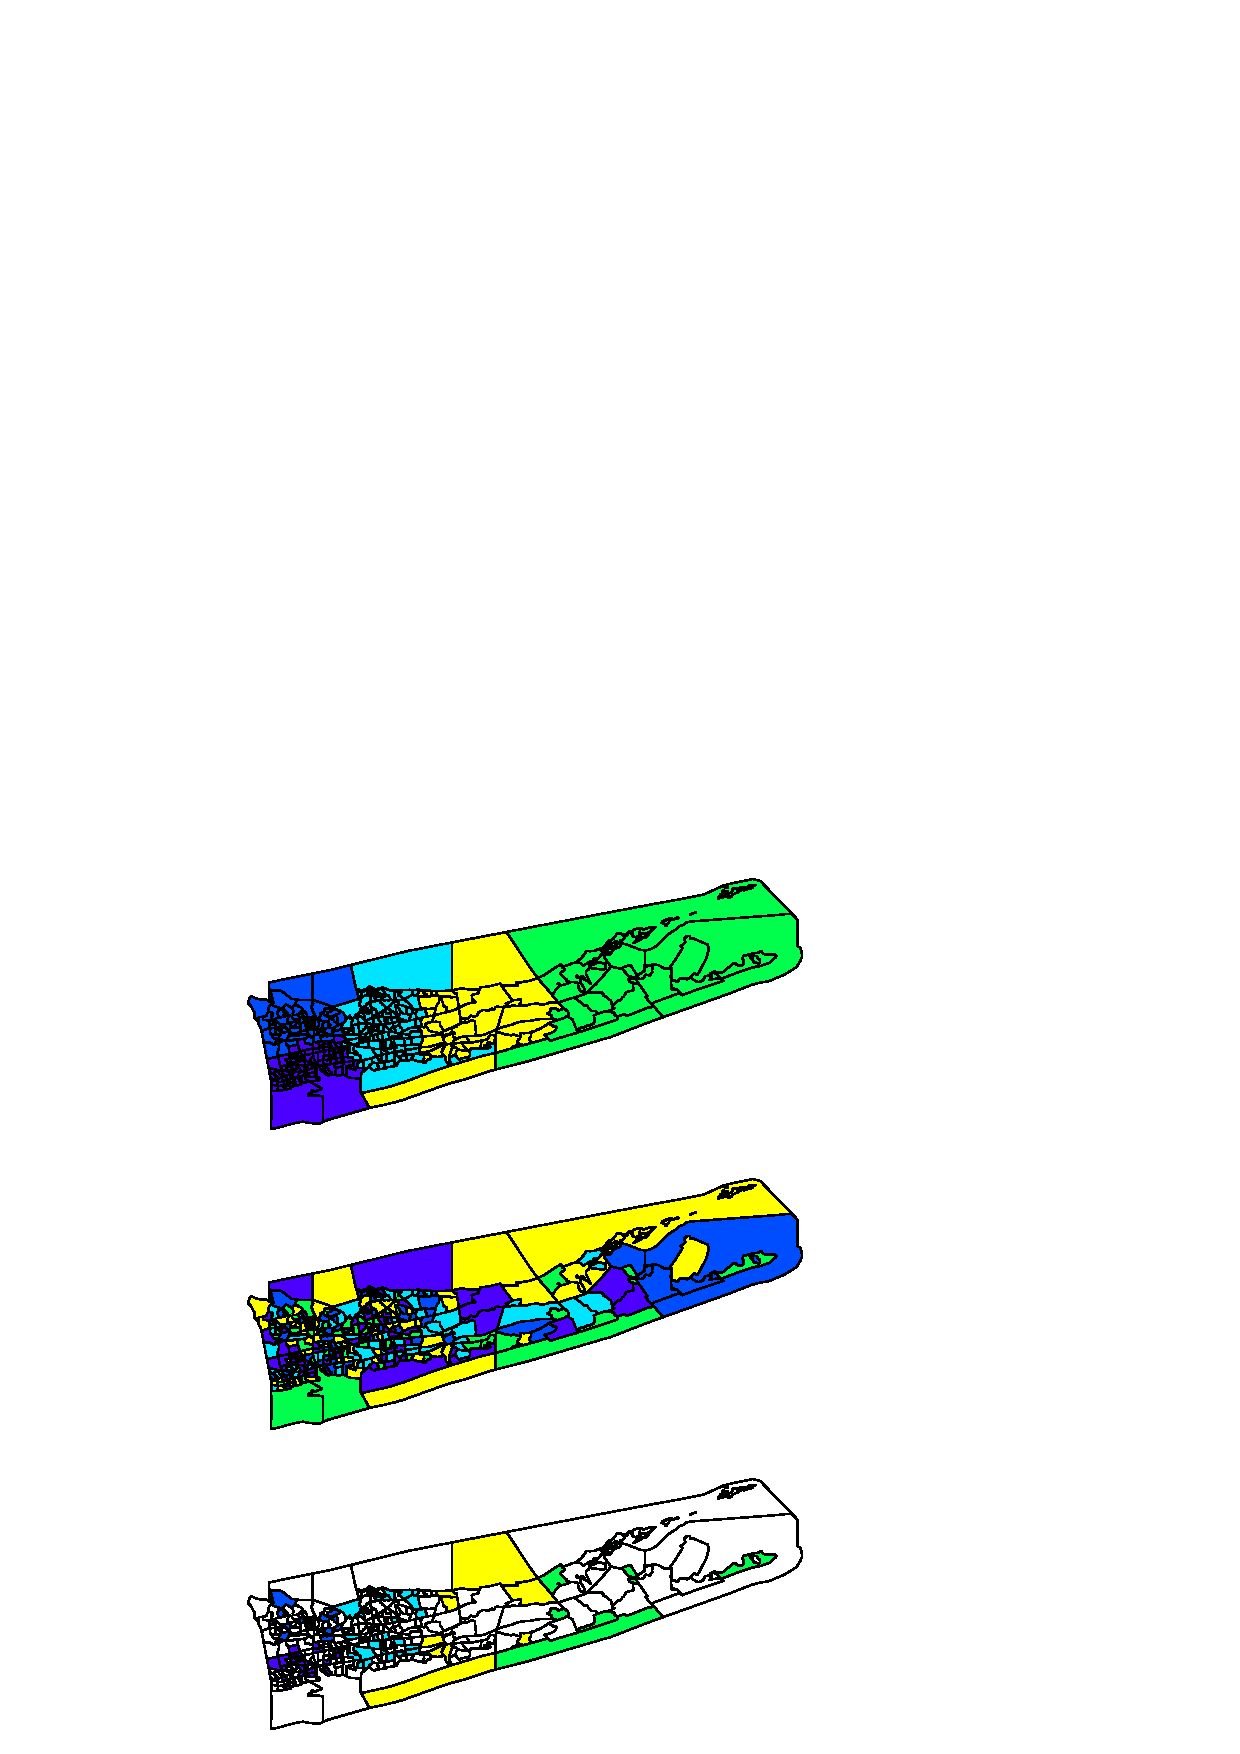
\includegraphics{bardJSS-plot2a}
  \caption{\label{fig:rplot2} Plotting differences among plans}
  \end{figure}
  
For reporting, \pkg{BARD} accepts user-generated score functions, which are discussed below. Additional plotting and reporting options are available and described in detail in the accompanying documentation.  

\section{A Mathematical Formulation of Redistricting Criteria}

When redistricting authorities draw district boundaries they do not 
simply take pen to paper (or mouse to mousepad).\footnote{Prior to redistricting, another process of \emph{reapportionment} is used to determine the number of districts to be drawn. We do not address reapportionment algorithms here. For more information see \citet{BalYoung01}.}  They also analyze information associated with the geographic 
components of districts to ensure that maps satisfy legal requirements and political realities. 
To solve redistricting problems with a computer, the analogous mathematical problem must be formalized.  Since redistricting 
intrinsically involves assigning discrete blocks of geography (or 
discrete individuals) to districts to achieve a set of goals that is a function 
of the redistricting plan as a whole, the corresponding mathematical 
problem thus falls into the general area of combinatoric optimization.\footnote{Generically, this formulation of the problem assumes that the fundamental units are indivisible. If units are divisible, the problem becomes a continuous optimization problem, and different approaches would apply. In practice, reaggregating census geography is difficult and uncertain (see, for example, \citet{ROAD}) the lowest level census geography is treated as indivisible in redistricting, with the rare exception of 'split blocks.' Blocks can be manually split, and \pkg{BARD} can proceed with plan evaluation and generation if a shapefile is generated that includes geographical representations of split blocks. Our software simply treats the input units as given -- so 'split blocks' can be included in the input data, although the software will not split blocks automatically.}

There are many ways to represent particular redistricting problems 
mathematically within the general combinatoric optimization 
framework \citep[][]{Altman97}. However, representing redistricting 
as a \emph{graph partitioning} problem is the most natural formulation, 
since it allows the expression of geographic values, such as compactness 
and contiguity in a simple and direct way. Furthermore, in previous 
research, this representation seems to be the most amenable 
to an efficient solution.\footnote{Less commonly, set-partitioning and integer programming 
approaches have been used to solve the redistricting problem. These 
are mathematically equivalent, although incorporating contiguity 
requires that a large number of side constraints be enumerated in 
formulating each problem instance. Also, geographic site-selection and 
facility allocation problems (as found in the operations research 
literature) are related to the redistricting problem, but no 
method is available currently to reformulate arbitrary 
redistricting problems in these terms. In terms of fundamental 
computational complexity, the particular problem representation is 
less important, since one could convert a redistricting problem 
instance back and forth among any different NP-complete problem 
representation in polynomial time. However, in practice, a proper 
choice of representation can make it much easier to formulate and 
solve the problem.In recent work,  integer programming approaches have been successsful in small problems  \citep[see][]{AerEisHeu03}, whereas success for much larger problems has bee reported using heuristics on graphs \citep[see][]{Xiao06}.}  

To put the problem in formal terms\footnote{For consistency, we use the notation previously published in \citet{Altman97} and \citet{AltmanThesis}.}:

\begin{enumerate}
\item Let \textbf{x}\textit{\textsubscript{i}} refer to the
\textit{i}\textsuperscript{th} census block, $\textit{x}\textit{\textsubscript{i}}\in{\textbf{X}}$ 
where \textbf{X} is the set of all census blocks in a jurisdiction. These blocks are
vector{}-valued, and we will assume that blocks are associated to various
population values, political measures, and geographic
locations, among other features.
\textbf{d}\textit{\textsubscript{j}} refers to the
\textit{j}\textsuperscript{th} district. \ A district is a set of
census blocks: 
% MathType!MTEF!2!1!+-
% feqaeaartrvr0aaatCvAUfeBSjuyZL2yd9gzLbvyNv2CaerbuLwBLn
% hiov2DGi1BTfMBaeXatLxBI9gBaebbnrfifHhDYfgasaacH8srps0l
% bbf9q8WrFfeuY-Hhbbf9v8qqaqFr0xc9pk0xbba9q8WqFfea0-yr0R
% Yxir-Jbba9q8aq0-yq-He9q8qqQ8frFve9Fve9Ff0dmeaabaqaciGa
% caGaaeqabaaaamaaaOqaaiaahsgadaWgaaWcbaGaamyBaaqabaGccq
% GH9aqpdaGadaqaaiaahIhadaqhaaWcbaGaamyAaaqaaaaakiaabYca
% caWH4bWaa0baaSqaaiqadMgagaqbaaqaaaaakiaab6cacaqGUaGaae
% OlaiaabYcacaWH4bWaa0baaSqaaiqadMgagaGbaaqaaaaaaOGaay5E
% aiaaw2haaaaa!40EC!
\[                                                    
{\bf d}_m  = \left\{ {{\bf x}_i^{} {\rm ,}{\bf x}_{i'}^{} ...{\rm ,}{\bf x}_{i''}^{} } \right\}
\]

\item 
\textbf{p}\textit{\textsubscript{k}} refers to a particular plan. plan
is a partition of the set of all census blocks \textbf{X} into a disjoint set of districts of exogenously given size $n$, such that ${\bf X} = \bigcup\limits_{\forall j} {{\bf d}_j^{} }$ and ${\bf d}_j \bigcap\limits_{\forall \left\{ {j,j'} \right\},j \ne j'} {{\bf d}_{j'} }  = \emptyset$:\footnote{A very small number of state and local jurisdictions permit 
overlapping ``floterial'' districts, which permit the assignment of units (typically towns or municipalities) to more than one district -- thus allowing voters in those municipalities to vote in multiple districts simultaneously.  BARD does not provide direct support for this situtation. In practice, this is often approached as a set of sequential partitioning problems: First partition the towns into $n-m$ districts. Then create a separate overlay partition of $m$ districts, using only `underepresented' towns. This sequential problem formulation could be solved using BARD, by removing ineligible units from the base map in the second stage.}
% MathType!MTEF!2!1!+-
% feqaeaartrvr0aaatCvAUfeBSjuyZL2yd9gzLbvyNv2CaerbuLwBLn
% hiov2DGi1BTfMBaeXatLxBI9gBaebbnrfifHhDYfgasaacH8srps0l
% bbf9q8WrFfeuY-Hhbbf9v8qqaqFr0xc9pk0xbba9q8WqFfea0-yr0R
% Yxir-Jbba9q8aq0-yq-He9q8qqQ8frFve9Fve9Ff0dmeaabaqaciGa
% caGaaeqabaaaamaaaOqaaiaahchadaWgaaWcbaGaamyAaaqabaGccq
% GH9aqpdaGadaqaaiaahsgadaqhaaWcbaGaamymaaqaaaaakiaabYca
% caqGUaGaaeOlaiaab6cacaqGSaGaaCizamaaDaaaleaacaWGUbaaba
% aaaaGccaGL7bGaayzFaaaaaa!3E5A!
\[
{\bf p}_i  = \left\{ {{\bf d}_1^{} {\rm ,}...{\rm ,}{\bf d}_n^{} } \right\}
\]
\item 
\textbf{G = (V,}\textbf{\textit{E}}\textbf{)} \textmd{is a mathematical
graph representing the underlying census block geography. Each} node
\textbf{v}\textit{\textsubscript{i}} in g represents a census block,
and each edge \textbf{e}\textit{\textsubscript{i,j}} denotes physical
adjacency of those block
\end{enumerate}

%\begin{figure}[!h]
%This figure provides a graphical illustration: 
%
% \begin{center}
%    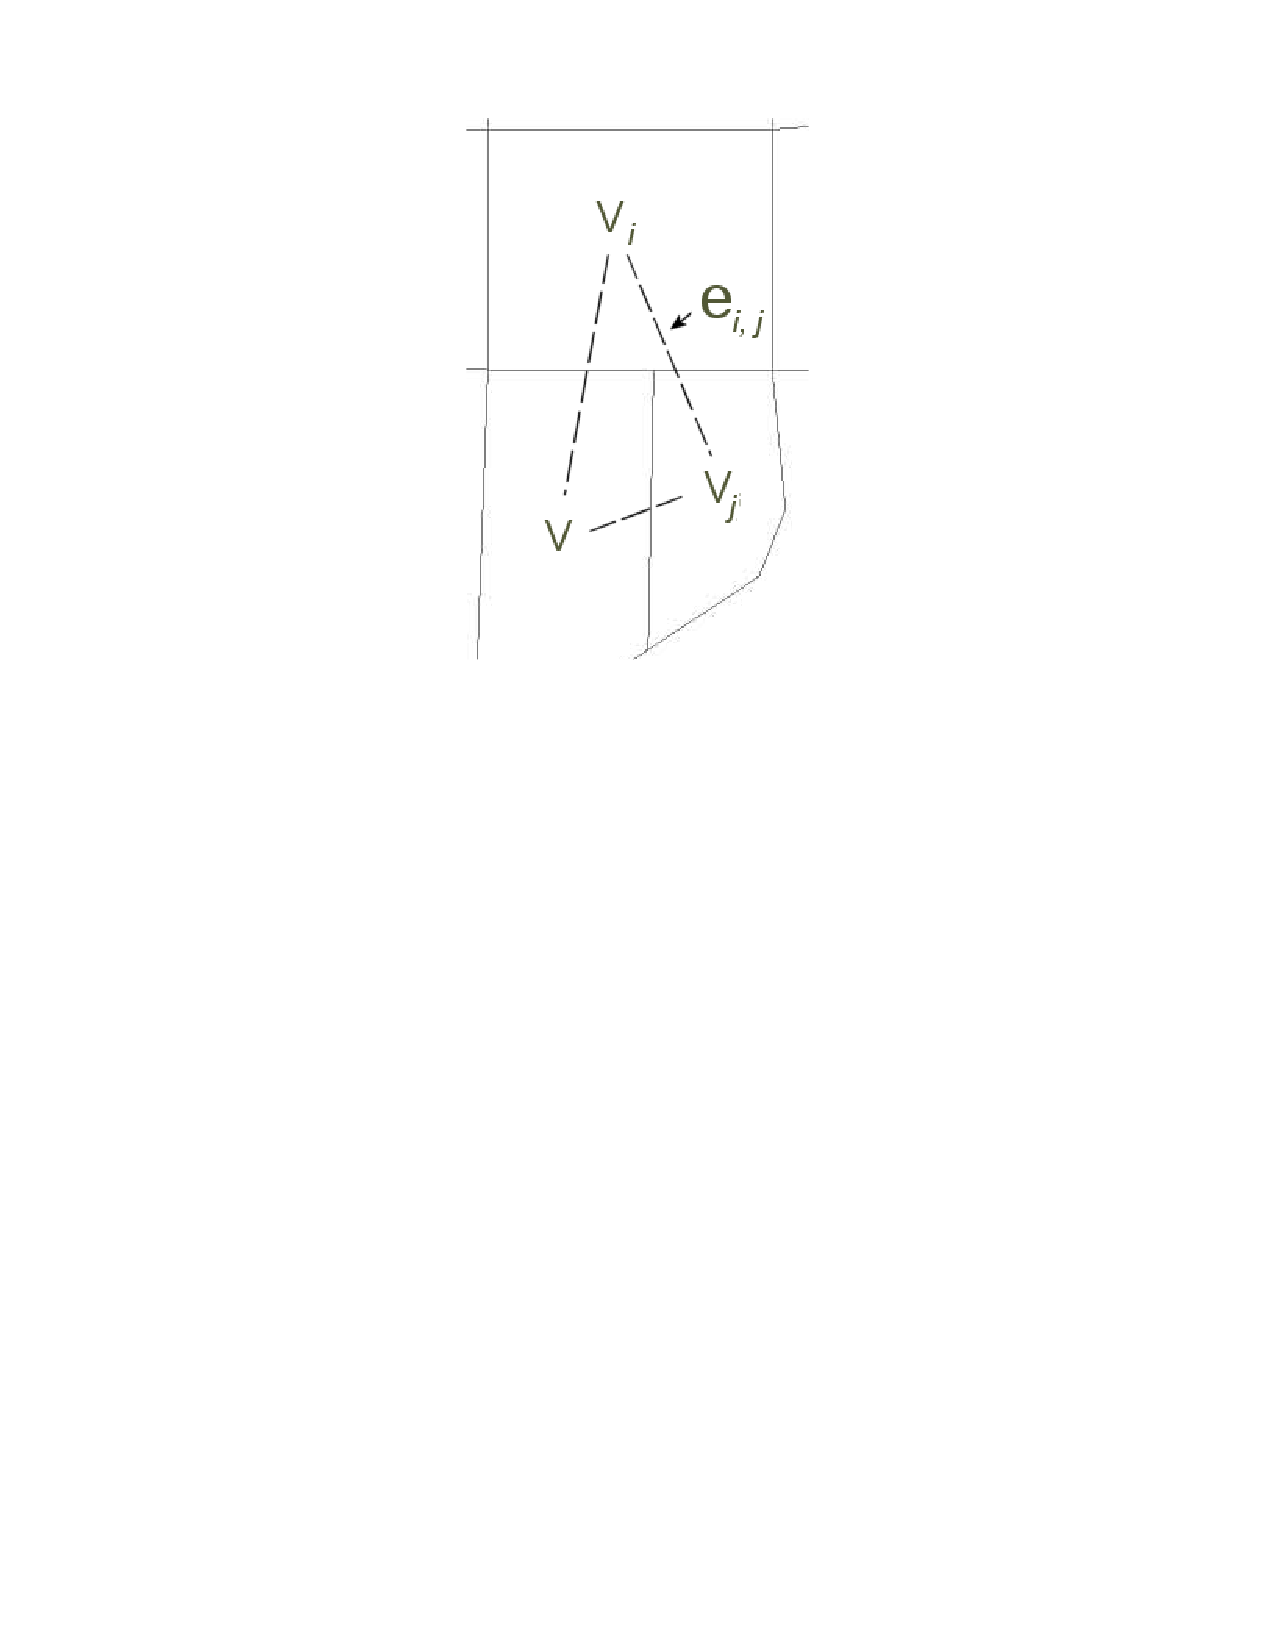
\includegraphics{fig_example.pdf}
%  \end{center}
%
%  \caption{\small Illustration of redistricting as a graph problem.}
%  \label{fig:example}
%\end{figure}

\subsection{Redistricting Criteria}

Part of solving this problem is operationalizing the criteria important 
for districting as functions of the demographic, political, and geographical 
properties of the redistricting plan. Here we discuss the most commonly recognized redistricting criteria \citep[see][]{McDonald04}, 
all of which can be easily calculated using score functions provided with \pkg{BARD}: equal population, 
completeness, contiguity, geographic compactness, political competitiveness or partisan bias, 
minority-opportunity to elect a candidate of choice, and 
respect for existing political boundaries or communities of interest.\footnote{Formally, required criteria for any legal redistricting plans, 
such as compactness, may be thought of as constraints rather than scores. 
In general in \pkg{BARD}, these constraints are treated as 
a very heavily valued component of the score function, thereby permitting the use of a variety of generalized optimization heuristics. However, a few (optional) specialized functions in \pkg{BARD}, such as the ``contiguous'' plan generation function, has one or more constraints ``hard-wired'' into the generation or refinement processes.} 

Perhaps the most important criterion is that districts 
 have equal population.\footnote{Congressional districts must be 
of less than a one percent population division to ensure that they 
conform to legal standards.  State legislative districts are 
permitted a ten percent population deviation under federal law, 
though some state laws require a smaller deviation \citep[][]{CainMacMc05}. In our software, both the score function for measuring population deviation, and the methods for generating initial district assignments allow the amount of tolerable deviation in population to be specified by the user.} And the format of population data released by the U.S. Census 
Bureau further guides how the redistricting problem is formalized.  
These data are not reported for individuals, rather, to protect the 
confidentiality of respondents data, these are aggregated into discrete 
geographic entities known as ``census blocks'' which roughly conform 
to a city block in urban areas. It is thus not difficult to imagine census blocks as corresponding to 
points on a graph.  

This conceptualization is how Geographic Information Systems (GIS) 
programs generally work: they plot the vertices of census blocks (and higher geographic 
units, such as counties and cities) onto a screen for user 
manipulation. GIS redistricting modules enable users to assign 
blocks to districts through simple point and click operations. 
Characteristic data associated with each block can be displayed 
on-screen.  For example, in the case of equal population 
requirements, blocks can be associated with their total population.  
If a district needs more population, a user can click on blocks 
adjacent to a district to identify those that will help meet a 
target population number.  GIS programs are well-suited to display 
and produce summary statistics of similar data, such as racial 
population data, which are used to meet target racial population 
numbers to conform with the Voting Rights Act, and election data, 
which are used to predict political outcomes. (Indeed, we might think 
of all such characteristic block data as belonging to the same 
family for optimization purposes.) However, GIS modules do not assure that the districts created in this way conform to criteria such as equal population, only that these data are available to map drawers.

Part of the definition of a legal redistricting plan is that it 
is a complete assignment of census blocks to districts. Thus completeness 
is not usually discussed explicitly as a redistricting criterion. Nevertheless, 
in practice, because of the technical complexity of redistricting, even professionals often commit errors leading to incomplete plans. To 
assist the creation of legal plans, \pkg{BARD} can evaluate the 
completeness of the proposed plan, and to repair ``holes'' in it. 

Another important criterion is that districts must (usually) be contiguous, or 
connected.\footnote{While contiguity is  a legal requirement in many states, it is
not a Federal requirement. And there are documented instances of 
non-contiguous districts or districts of questionable contiguity because 
they are connected over water without a bridge \citep[][]{Altman98}.  
Another example, some states require districts to be composed entirely 
of wards or other political subdivisions which are themselves sometimes non-contiguous when odd city boundaries create islands of 
incorporated or unincorporated territory.  The Wisconsin 61\textsuperscript{st} Assembly district created in 2001 is non-contiguous 
as a result of containing such a ward on its perimeter.  To 
avoid having non-contiguous districts, the state created a legal 
fiction that states all wards are contiguous, see Wisconsin Code 5.15(1)(b)}   
The geospatial coordinate data used to plot census blocks can also be used to determine if two blocks are connected to one another.  In normal operation,
block boundaries are pre-processed to generate a complete contiguity matrix that  
lists every block's neighbors which \pkg{BARD} then uses to determine rapidly if 
a proposed plan satisfies contiguity.

Geographic compactness is an oft-mentioned criterion for redistricting 
that is honored in the breach.  Dozens of scores have been proposed, but 
few are used in practice (see \citet{Altman98}, \citet{Niemi91}). \pkg{BARD} provides three functions that calculate common geographic compactness scores which capture the dispersion and dissection of districts (how much they are stretched or have chunks removed from them). \pkg{BARD} also provides a parameterized and weighted `moment-of-inertia' score that can be used to measure geographic compactness, population compactness, and cumulative distance from fixed locations, such as candidates homes, warehouses, or schools. Other scores can easily be programmed in \proglang{R}.

Election outcomes that may be expected from a redistricting plan can be constructed from election or demographic input variables. Estimates of how reliably 
districts may elect partisan candidates of either party are commonly measured by estimating the expected partisan vote share in each districts \citep{McDonald06a}.\footnote{An alternative way of evaluating the political outcomes of the plan involve estimating the predicted seat-votes curve resulting from that plan. This was proposed thirty years ago 
by \citet{Tufte73} and \citet{NieDee78}. \citet{GelKing94} provide the leading method for estimating this.} 
If the expected ratio of partisan vote shares is approximately the same within a threshold tolerance, a district is deemed competitive by this measure. 
In a similar manner, minority opportunity districts are usually identified as those in which the ratio of minority 
population to majority population falls above a designated threshold \citep{GrofHand92}.
These partisan or racial vote share may be estimated simply, based on voter registration in the proposed 
district, or through a more complex model such as in \citet{GelKing94}.  The \pkg{BARD} 
framework provides a generalized scoring function that efficiently computes the sum of a predictor variable 
associated with each block, or the ratio of two predictive variables. With this it is 
possible to calculate estimates of the number of districts that may be won by a party's candidates, district competitiveness scores, 
identify minority-opportunity districts, or other predictive election results.  

Another quasi-geographic set of criteria often found in state law is  
`respect' for geographic or political features such as city or county 
boundaries, communities of interest (often defined by redistricting 
authorities), or other `natural'  features such as rivers or mountain ranges.  
Capturing these criteria mathematically is straight-forward: any set 
of census blocks can be defined as belonging to a grouping set and
a penalty for splitting groups can be added to the score function for evaluating a redistricting plan.\footnote{We are sympathetic to the argument put forth by \citet[][]{Forest04} 
that using only quantitative data to represent communities of interest can result
in `thin' representations of community. Using the technique just described, the \pkg{BARD} system can incorporate
information about the boundaries of communities of interest based on external qualitative 
analysis and ``thick'' descriptions.}  An example of this type of community cost 
function is included in the \pkg{BARD} package.  The twist is that these criteria are 
often secondary to equal population, contiguity, and Voting Rights Act concerns, and so the scores
associated with each criterion must be properly weighted in order to permit 
some violation of feature boundaries to accommodate superseding criteria.
All of these criteria may be calculated in \pkg{BARD}.

In addition, the \pkg{BARD} score framework enables any function of model in \pkg{R} to be used in the evaluation of 
a plan. Thus, it is relatively straightforward to add new scores to \pkg{BARD} to evaluate plans 
based on the user's choice of statistical model.
%such as cross-level inference model 
%estimates of voter behavior (e.g., using \pkg{eco} or  models predicting 
%election results or seat-votes curves such as \pkg{JudgeIt2} --  see %\citet{Imai07} and \citet{GelKing07}, respectively).

We note that there is no universally agreed upon set of redistricting criteria, and many jurisdictions
often require vague goals such as ``compact'' districts, without a specific definition to
guide implementation. For example, is compactness defined as the minimization of the 
length of the district perimeter or the ratio of the district's area to that of the largest inscribed circle
(both are proposed methods of measuring compactness)?  Different formulations may lead to substantively
different types of districts, which means that redistricting criteria may have subtle
``second-order biases'' \citep[][]{Parker90}, that is, the criteria are seemingly 
neutral on face value but reliably produce a political outcome.  Defining criteria 
and meaningfully weighing them against one another is an art that demands experimentation 
since no two jurisdictions have the same geography or population distribution.  This 
also reveals the importance of the \pkg{BARD} open source approach to formulating redistricting criteria (and automation) 
since a black box approach is vulnerable to hidden manipulation.  

\section{Use of Automated Redistricting for Plan Analysis}

In addition to evaluating and improving existing plans, automated redistricting 
has long been used as a method for redistricting analysis, especially by political geographers.  Pioneering work by 
\citet{ShepJen70} and \citet{GudgTayl79} employ enumeration of all 
possible partitions (for extremely small districting plans) to reveal the complete range of possible redistricting alternatives.  

Scholars have proposed methods other than full enumeration to overcome the computational limitations of enumeration on even modestly 
redistricting problems, with as little as 50 units to assign to districts.  Another way of using automated redistricting for analysis is taken by \citet{Altman97} and \citet{RogersonYang99}. These authors propose 
automated refinement of redistricting plans to simulate the effects of additional legal constraints on redistricting outcomes.  Another alternative, 
and relatively common use of automated redistricting, is to use ``random'' generation of 
districts to probe the characteristics of arbitrary redistricting plans (see \citet{EngWild77,RosJohn81,Oloughlin82,Grofman82,CirDarOro00}). 
Note however that work does not establish that `random' districts are probability samples from a well-described population of plans  \citep{AltmanMcDonald04}. \footnote{For example
\citet[e.g.,]{CirDarOro00} use a random-walk like method to create contiguous districts. However, the process can be shown not to yield a simple random sample of redistricting plans in small samples, and indeed there is no evidence to establish convergence to a probability sample.  In general, as Knuth warns, algorithms that are stochastic do not necessarily yield 
random distributions of results \citep[][]{Knuth97}. 
} We recommend that these methods be interpreted with caution.


\section{Improving Algorithms for Automated Redistricting Refinement} 

The \pkg{BARD} package provides functions to refine districts based on specified score functions. In this section we describe the formulation of the refinement problem, existing software, and the algorithms \pkg{BARD} currently provides.  

Formally, redistricting is a computationally complex optimization 
problem: Common variations of redistricting be shown to be equivalent to general optimization problems already  known to be `NP-Complete'  \citep[see][]{Altman97}. An illustration of this is the specific problem of finding equi-populous contiguous plans. Formally, this is equivalent to the the following optimization problem, known as
``\textbf{Cut into Connected Components of Bounded Size (\& Weight)''} \citep[][]{Johnson1982}: 

\emph{Is there a partition of vertices}, \textbf{V,}\textit{ } \emph{into disjoint
sets} \textbf{V}\textit{\textsubscript{1 }}\emph{and}
\textbf{V}\textit{\textsubscript{2}} \emph{such that} 
% MathType!MTEF!2!1!+-
% feqaeaartrvr0aaatCvAUfeBSjuyZL2yd9gzLbvyNv2CaerbuLwBLn
% hiov2DGi1BTfMBaeXatLxBI9gBaebbnrfifHhDYfgasaacH8srps0l
% bbf9q8WrFfeuY-Hhbbf9v8qqaqFr0xc9pk0xbba9q8WqFfea0-yr0R
% Yxir-Jbba9q8aq0-yq-He9q8qqQ8frFve9Fve9Ff0dmeaabaqaciGa
% caGaaeqabaaaamaaaOqaamaaqafabaGaae4CamaabmaabaGaamODaa
% GaayjkaiaawMcaaaWcbaGaamODaiabgIGiolaahAfadaWgaaadbaGa
% amymaaqabaaaleqaniabggHiLdGccqGHKjYOcaWGlbaaaa!3E1C!
\[
\sum\limits_{v \in {\bf V}_1 } {{\rm s}\left( v \right)}  \le K
\]
 and 
% MathType!MTEF!2!1!+-
% feqaeaartrvr0aaatCvAUfeBSjuyZL2yd9gzLbvyNv2CaerbuLwBLn
% hiov2DGi1BTfMBaeXatLxBI9gBaebbnrfifHhDYfgasaacH8srps0l
% bbf9q8WrFfeuY-Hhbbf9v8qqaqFr0xc9pk0xbba9q8WqFfea0-yr0R
% Yxir-Jbba9q8aq0-yq-He9q8qqQ8frFve9Fve9Ff0dmeaabaqaciGa
% caGaaeqabaaaamaaaOqaamaaqafabaGaae4CamaabmaabaGaamODaa
% GaayjkaiaawMcaaaWcbaGaamODaiabgIGiolaahAfadaWgaaadbaGa
% aGOmaaqabaaaleqaniabggHiLdGccqGHKjYOcaWGlbaaaa!3E22!
\[
\sum\limits_{v \in {\bf V}_2 } {{\rm s}\left( v \right)}  \le K
\]
\emph{and both}
\textbf{V}\textit{\textsubscript{1 }}\emph{and}
\textbf{V}\textit{\textsubscript{2}} \emph{induce connected subgraphs of}
\textbf{G}\textit{?}
\\
For very small numbers of vertices, the optimal plan could be selected simply by enumerating all feasible redistricting plans and identifing the most optimal plan.  
Unfortunately, for the task of redistricting a state's congressional 
or state legislative districts, no algorithm is guaranteed success 
in a reasonable time.  Consider a middle-sized state such as 
Wisconsin, which has slightly more than 330,000 census blocks.  If 
blocks were of equal population, then there would be more possible redistricting 
plans than there are quarks in the universe.  More generally, the number of
possible districts for a given number of equi-populous blocks and districts 
is a Stirling Number of the Second Kind:

% MathType!MTEF!2!1!+-
% feqaeaartrvr0aaatCvAUfeBSjuyZL2yd9gzLbvyNv2CaerbuLwBLn
% hiov2DGi1BTfMBaeXatLxBI9gBaebbnrfifHhDYfgasaacH8srps0l
% bbf9q8WrFfeuY-Hhbbf9v8qqaqFr0xc9pk0xbba9q8WqFfea0-yr0R
% Yxir-Jbba9q8aq0-yq-He9q8qqQ8frFve9Fve9Ff0dmeaabaqaciGa
% caGaaeqabaaaamaaaOqaaiaadofadaqadaqaaiaad6gacaGGSaGaam
% OCaaGaayjkaiaawMcaaiabg2da9maalaaabaGaaGymaaqaaiaadkha
% caGGHaaaamaaqahabaWaamWaaeaadaqadaqaaiabgkHiTiaaigdaai
% aawIcacaGLPaaadaahaaWcbeqaaiaadkhaaaGcdaqadaqaaiaadkha
% cqGHsislcaWGPbaacaGLOaGaayzkaaWaaWbaaSqabeaacaWGUbaaaO
% WaaSaaaeaacaWGYbGaaiyiaaqaamaabmaabaGaamOCaiabgkHiTiaa
% dMgaaiaawIcacaGLPaaacaGGHaGaamyAaiaacgcaaaaacaGLBbGaay
% zxaaaaleaacaWGPbGaeyypa0JaaGimaaqaaiaadkhaa0GaeyyeIuoa
% aaa!5408!
\[
S\left( {n,r} \right) = \frac{1}{{r!}}\sum\limits_{i = 0}^r {\left[ {\left( { - 1} \right)^r \left( {r - i} \right)^n \frac{{r!}}{{\left( {r - i} \right)!i!}}} \right]} 
\]

In practice, contiguity will 
reduce the number of feasible plans that must be enumerated, none-the-less, the number 
of possible plans likely remains staggeringly large.  Thus, 
selecting the globally optimal plan from a full enumeration of all 
plans is not feasible even using the fastest computers currently available. For similar reasons, random generation of districting plans (e.g. via a random walk) is unlikely to generate feasible plans. 

Lacking enumeration, some sort of heuristic or algorithm is needed to find an 
optimal redistricting plan. The fact that the problem has been shown to be NP-Complete strongly suggests that there are no efficient algorithms capable of solving the problem with any guaranteed approximation of optimality. Thus researchers in this area have turned to heuristic approaches, that while not guaranteed to produce quality solutions, do complete in a reasonable amount of time. 

A variant on simple random block assignment is a ``greedy'' 
heuristic that starts from a seed block and randomly assigns 
additional contiguous blocks to a district until a target population 
value is reached. Perhaps a greedy algorithm could find an optimal redistricting plan 
if there was one clear path to the optimal plan.  Upon reflection, this is unlikely to  
 work for most redistricting problems.  For example, imagine a state must draw a district 
with more than a majority percentage of minorities 
(so called ``minority-majority'' districts) to be in 
compliance with the Voting Rights Act.  Imagine that there are two 
sizable minority communities separated by a white 
suburb.  The only feasible minority-majority district is one that 
links the communities by a narrow bridge across the suburb.  A 
greedy algorithm aimed towards maximizing district minority 
population might easily miss this arrangement because  
drawing a bridge across the white community would momentarily decrease the value of the objective
function to be maximized until the bridge was complete. In general, partitioning problems such as the redistricting problem are known to be rife with local optima that trap greedy approaches.\footnote{Note that the final target of the heuristic must be generation of a plan. Since the allocation of one district affects others in the same plan, heuristics that take a district-by-district approach are even more prone to being trapped at local optima. }

%As might be expected from the theoretical computational complexity 
%of the problems, exact (optimal) methods have been 
%unsuccessful in yielding solutions to problems of significant size. 
%The most successful of the exact solution methods, based on 
%integer-programming formulations, have advanced considerably over 
%the last decade, but are still limited to relatively small problems: 
%In a recent study a redistricting problem on a 30x30 grid was solved  
%\citep[][]{AerEisHeu03} for a fixed set of redistricting 
%criteria, and the authors speculated that such methods could be 
%extended up to a 50x50 grid. 

%Exact solution methods are difficult or impossible to extend to 
%arbitrary redistricting criteria. Even integer programming, which is 
%one of the most (if not the most) general formulations for which 
%exact solution methods are used, requires extensive expertise to reformulate 
%redistricting criteria as integer partition constraints.  In contrast, success 
%using evolutionary algorithms. on artificial grid data of up to 
%500x500 has been reported for a related site-search allocation 
%problem 


\subsection{Available Software}

Despite a long history of experiments in automated redistricting, 
there are few tools publicly available for automated redistricting. 
To our knowledge, five commercial software tools produced by Caliper 
Corporation, ESRI, Digital Engineering Corporation (which provides 
a redistricting add-on for ESRI's GIS program), Corona Solutions, 
and Manifold Systems provide automated redistricting functionality 
\citep[][]{AltMacMcD05}.\footnote{In addition to these companies, 
the Texas Legislative Council developed prior to the 2001 round of redistricting a promising in-house 
automated redistricting program known as TARGET with limited exploratory
capabilities.}   

All publicly available tools are limited in several regards.  
They are capable only of producing districts with equal 
population and have no means to accommodate other criteria necessary 
to produce legal plans. All but one program uses variations on 
steepest ascent heuristics, the exception is Corona Solutions which 
claims to use a single-criterion genetic algorithm.  Unfortunately, 
we do not know much about the internal workings of these programs since they are 
closed-source and their algorithmic details poorly documented, which raises transparency issues similar to the controversies surrounding 
electronic voting machines.  These redistricting GIS programs with automated algorithms typically 
cost several thousand dollars (Manifold being the single notable exception), limiting their wide use.  

In our testing of these programs (see \citet{AltMacMcD05}), we found that while they could generate plans of a sort automatically, these plans would not satisfy legal requirements or basic plausibility. 
For example, ESRI's automated redistricting algorithm stops growing districts when the growing circular districts touch, yielding polka-dot districts that leave much of a jurisdiction unassigned to any district. Manifold's algorithm apparently randomly selects a number of blocks equal to the number of districts as seeds and grows districts from these seeds one district at a time, thereby sometimes producing a single-block district when other districts are first grown around it. 

Moreover, these programs are limited to balancing the allocation of a single fixed variable (measured at the unit level), sometimes in combination with a built-in (and usually idiosyncratic) measure of compactness, using a single optimization methods. These programs cannot perform multi-criteria optimization, accept user-defined weights and score functions, use alternative definitions of compactness, or probe trade-offs between the redistricting criteria and political goals. Thus, for most of the redistricting scenarios that \pkg{BARD} is intended to address, the available commercial automated redistricting software simply cannot be applied.

That these companies supply rudimentary automated features is perhaps unsurprising,  since there is little \emph{market} demand for automated functionality. Well-funded redistricting authorities and consultants are reticent to hand over highly sensitive political decisions to a machine. They have little incentive to use this functionality, since they can accomplish their ends without it, and it exposes them to potential legal complications since their optimization goals would be made clear. Although there is no money in it (and hence no market), public participation in the process will, however, be aided by these functions since they make it easier to draw plans that meet legal constraints and serve public goals.

\subsection{New Metaheuristic Approaches} 

A more general optimization heuristic is needed to address the redistricting problem. To be adaptable to any
reasonable redistricting goal, a successful approach should consider not only additions 
of single census blocks to a district core, but also arbitrary exchanges of multiple blocks among districts.  
To avoid being trapped in local optima, such a heuristic must be permitted to make 
some backwards (non-improving) steps in search of the global optimum, such as 
bridging two minority communities through a white community. These features 
of the redistricting problem suggest that \emph{metaheuristics} may be an effective practical solution.
 
Over the last two and a half decades, a set of new and surprisingly 
effective heuristic approaches to large optimization problems have 
arisen, including simulated annealing, evolutionary optimization 
(including genetic algorithms), iterated local search (including 
greedy randomized adaptive search), ant colony optimization, and 
tabu search.  These approaches, although formulated independently, 
have now been recognized as belonging to a more general \emph{metaheuristic} framework.

Essentially, metaheuristics are a general approach to optimization that involves 
combining a set of basic heuristics that find optima only in a local neighborhood with a 
larger framework for guiding and applying these heuristics 
repeatedly in a large search space (see \citet{BlumRoli03} for an in-depth 
survey of metaheuristics, and \citet{Altman97} \citet{CortonaEtAl99} and 
\citet{Xiao03} for other optimization algorithms used in redistricting).  
Designing and applying metaheuristics requires dynamically 
balancing between \emph{diversification}  and \emph{intensification}. Diversification involves generating new 
candidate solutions in such a way as to thoroughly explore the solution space. Intensification involves using (implicitly or explicitly) 
the history of candidate solutions that have been previously evaluated to guide the direction of an iterative search. 
Diversification is needed to have a high probability of finding the region of solutions that contains an optimal solution 
and intensification is needed to find these solutions in a practical amount of time. 

These metaheuristics have many variants and parameterizations, and none work well for all optimization problems \citep[][]{WolMac97}. This raises the possibility of  `third-order' bias, in which attributes of the outcome not specified in the optimization function may be affected in systematic ways by the solution method \citep[][]{Altman97}. Finding the right solution approach for a particular domain of problems is a matter of craft as much as science. Although no single metaheuristic is guaranteed to be ideal, there are many reasons 
why the metaheuristic framework is an appropriate one to use for redistricting:
\begin{enumerate}
\item First, metaheuristics have a track record of being successful on difficult combinatoric 
optimization problems. Redistricting is an exemplar of such a problem -- no sure solutions 
are available and no sure solutions are likely to be discovered due to the problem's computational complexity.
\item Second, in experimental work metaheuristics are most successful 
for redistricting-like partitioning problems.
\item Third, metaheuristics do not assume \emph{a-priori} a set of 
particular redistricting goals, or operationalization of them (although 
it is still likely that a particular configuration of selected metaheuristic is better at optimizing on one
type of goal, such as compactness, than another, such as competitiveness). 
By using a general metaheuristic framework we can allow the redistricting plan's author 
the flexibility to specify goals to be satisfied, rather than hard-coding the
goals into the solution method.
\item Fourth, by using multiple metaheuristics to ``solve'' the same problem, 
we reduce the threat that a particular heuristic can systematically interact 
with a redistricting goal to bias the resulting plan.
\end{enumerate}

\subsection[Optimization Methods in BARD]{Optimization Methods in \pkg{BARD}}

The initial version of \pkg{BARD} includes four metaheuristics: 

\emph{Simulated Annealing} (see citations above) exploits an analogy between the
way in which molten metal freezes into a minimum energy
crystalline structure (the annealing process) and the search for a
function optimum.  At each iteration, simulated annealing randomly generates
a candidate point (or set of points) within a local neighborhood
of the current solution. The probability of moving from the
current solution to one of the candidate points is a function of both
the difference in the value of the objective function at each point, and a 
temperature parameter. At high temperatures, candidate points that are ``worse'' than 
the current solution can be selected as the solution in the next iterate.  This helps the 
heuristic to avoid a local optimum. At each iteration, the temperature is reduced gradually, so 
that the probability of heading downhill becomes vanishingly small.

\emph{Genetic Algorithms} (see citations above) are a form of heuristic inspired by analogies 
between optimization (and adaptation) and the evolution of competing
genes.  In a genetic algorithm, a population set of candidate solutions are supplied to the optimization problem. 
Each solution is encoded as a string of values. At each iteration each member of the population is subject, at random, 
to mutation (an alteration of the solution vector), hybridization (a reshuffling of subsequences between two solutions). 
In addition, each round undergoes selection, where some solutions are discarded and some are 
duplicated within the population, depending on the fitness (function evaluation) of that member.

\emph{Tabu Search} (see \citet{Glover86} and the citations above) modifies hill-climbing by retaining a memory of recent moves (or attributes thereof) and avoiding those moves unless they meet particular aspiration criteria. This use of memory encourages diversification.

\emph{Greedy Randomized Adaptive Search} or GRASP \citep{FeoRes89} is a multi-start metaheuristic. Each iteration 
involves two phases, generation of a random starting candidate solution, and greedy exploration of 
the search neighborhood (hill-climbing) to find a local optimum. GRASP iterates repeatedly, and 
returns the best solution across all iterations. 

Greedy algorithms, when applied to redistricting problems, almost inevitably become trapped at a local optimum. The performance of such heuristics 
performance is thus quite sensitive to starting values. This is true even for 
metaheuristics unless the researcher is lucky, adapts the heuristic to the particular problem successfully, or uses external knowledge to pick starting values in the correct basin of attraction for the global optimum. Solving difficult optimization problems, however, is as much an art as a science.   

A problem's difficulty is increased when trying to optimize on multiple constraints, for 
example equal population and contiguity. A solution that scores well on equal population may 
have difficulty improving districts to create a plan with contiguous districts.  When a plan has 
near equal population, but is not contiguous, the rearrangement of blocks to create a contiguous plan 
may first require large negative steps on equal population before population re-balancing can resume to
produce a plan that is both contiguous and has equal population.

The proceeding example suggests that the size of the local neighborhood being searched at each iteration affects optimization performance.
Sometimes an algorithm must take large steps to escape a local optimum's basin of attraction. 
For example, a simulated annealing algorithm that considers only a single trade of census blocks among districts at each iteration 
may become trapped in a local optima more easily than one that considers trades of two or more blocks at a time.   However, considering local neighborhoods induced by multiple rather than single trades makes these neighborhoods much larger, and  more difficult or impossible to search thoroughly (ruling out some forms of greedy heuristic, for example.)
	
Selecting good starting values makes it much easier for metaheuristics to yield improved plans.  
In practice, when one starts with a current legal plan, it is much faster to generate a new, better-scoring plan 
than when starting from entirely randomly generated districts.  A potential problem with using the former districts as a starting point is that the same
political motivations that predominate the district shapes may continue to influence the solution.  

\section{Plan Refinement, Sampling and Profiling}

This simple demonstration shows how \pkg{BARD} can be used to repeatedly generate and refine plans by applying one optimization algorithm to a set of 21 plans: a plan generated by k-means plus 20 plans generated by \code{createRandomPlan}. Each plan is then refined using the score function and optimization function indicated:

\begin{Schunk}
\begin{Sinput}
> myScore <- function(plan, ...) combineDynamicScores(plan, scorefuns = list(calcPopScore, 
+     calcLWCompactScore))
> samples <- samplePlans(list(kplan), score.fun = myScore, ngenplans = 20, 
+     gen.fun = "createRandomPlan", refine.fun = "refineNelderPlan", 
+     refine.args = list(maxit = 200, dynamicscoring = TRUE))
\end{Sinput}
\end{Schunk}

This yields a set of improved plans, which can be summarized and plotted using methods that the package supplies for evaluating \emph{groups} of plans. \pkg{BARD} also supplies a \code{profilePlans} function that replicates samplePlans, while reweighting components of a given score function. This allows one to examine the effects of trade-offs among pairs of redistricting criteria. 

  \begin{figure}[!h]
\begin{Schunk}
\begin{Sinput}
> plot(summary(samples))
\end{Sinput}
\end{Schunk}
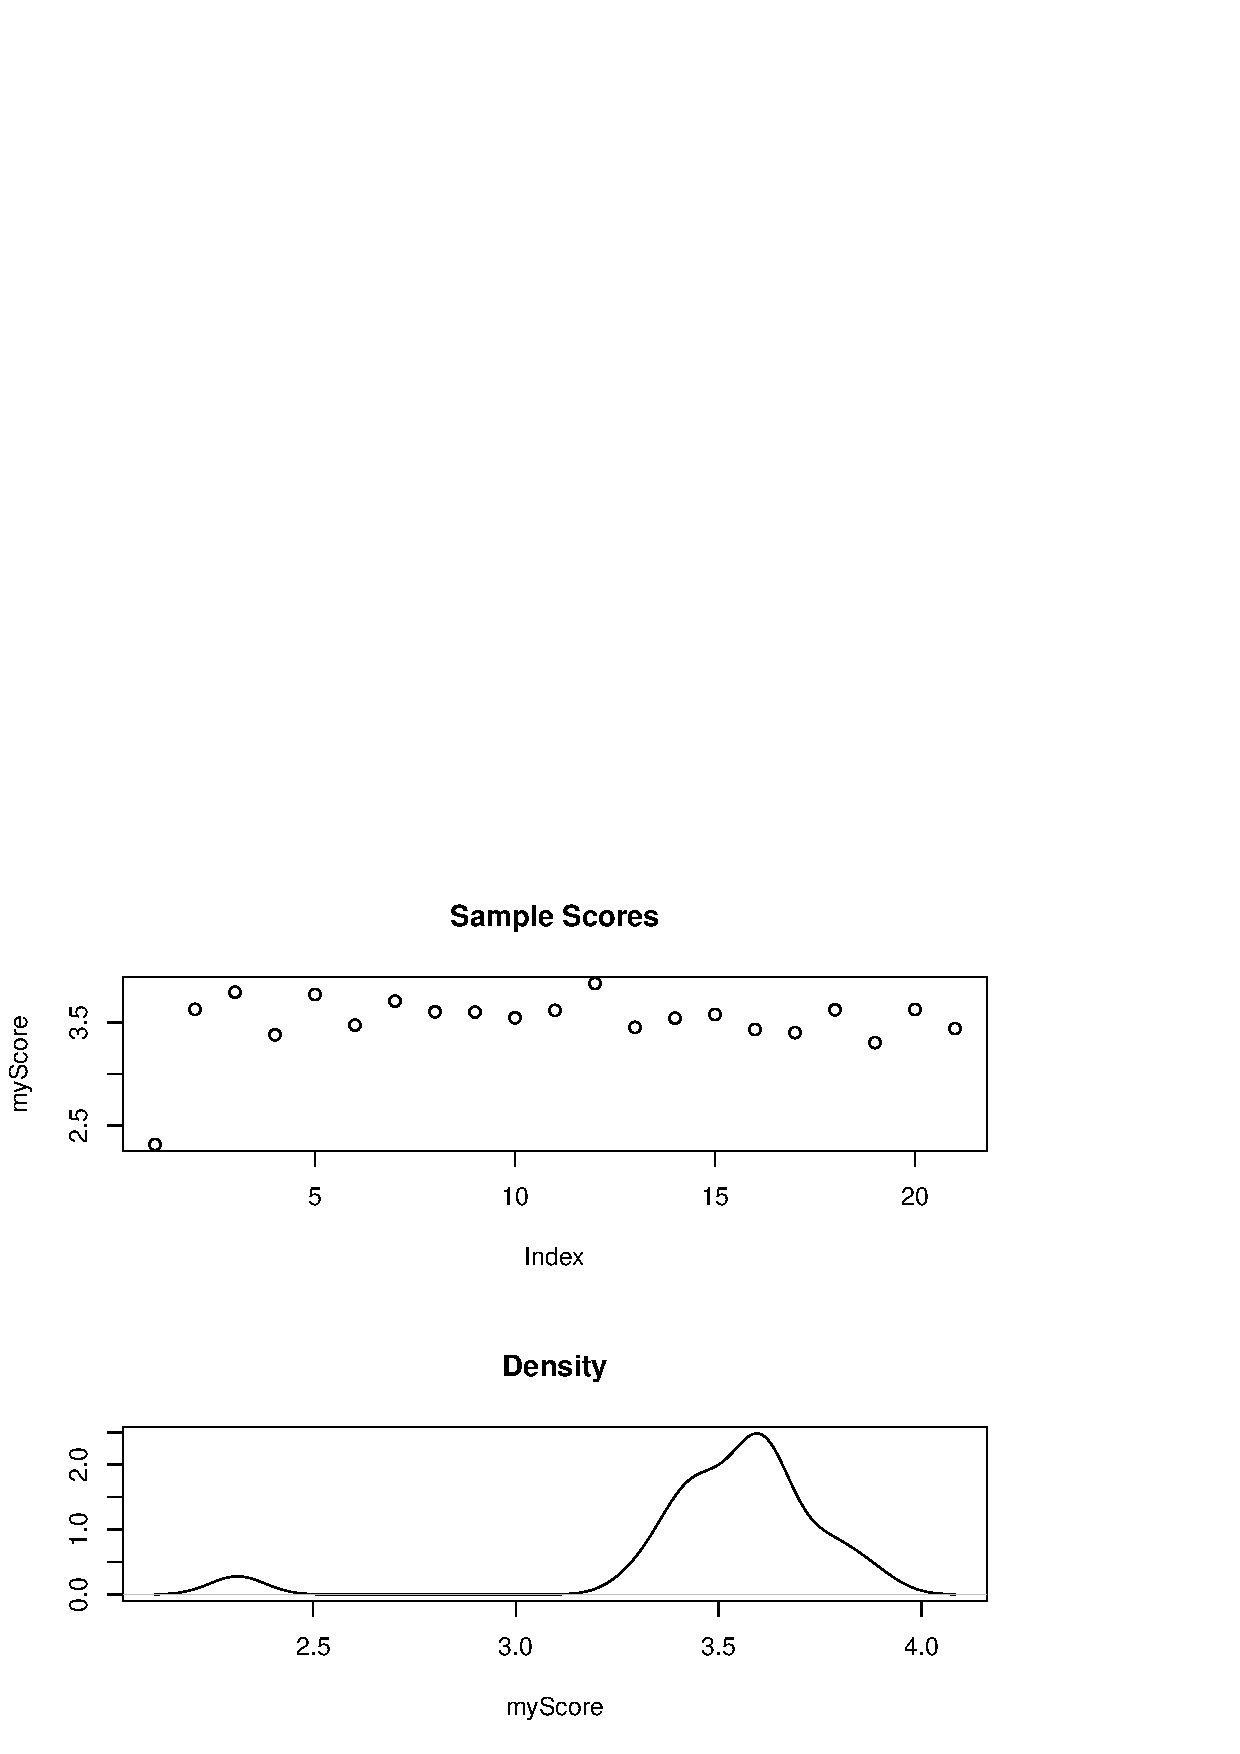
\includegraphics{bardJSS-plot3a}
  \caption{\label{fig:rplot3} Plotting a distribution of ``samples'' randomly generated districts}
  \end{figure}
  
Although redistricting is a computational problem that is too difficult to ensure the resulting plan is \emph{optimal}, the program may yield a useful improvement over the starting map and may further enable the public to generate constitutionally viable plans. \footnote{To keep the run-time of this demonstration manageable, we implement the essential profiling steps  using a quick but primitive optimization method, \code{refineNelderPlan}.  In a real (and long running) application we would substitute \code{refineTabuPlan}, \code{refineAnnealPlan}, \code{refineGRASPplan}, or \code{refineGenoudPlan} for \code{refineNelderPlan} above.}  

A unique aspect of \pkg{BARD}'s approach is that it enables
one to explore the tradeoffs between redistricting goals, such as the
de-minimis population inequality effect and district
compactness, the creation of an additional majority-minority
district, the number of partisan seats and district
competitiveness, and compactness. We can repeatedly
generate plans using the same set of redistricting goals,
while systematically changing the weight given to
one (or more) of those goals. For example, if plans generated
using a scoring rule that weights compactness heavily have
significantly fewer minority districts than plans generated with a
lower weight on compactness, this suggests a tradeoff exists
between compactness and minority representation.

A variant of this technique can be applied to reveal the
preferences of those who created a districting plan. Informally, if we
start with a redistricting plan chosen by a set of participants and
show that a small modification to this plan has a large impact on 
a particular goal without much affecting other relevant criteria, we can infer that the plan's author places a relatively low
value on that goal. For example, if a more competitive plan can be produced at the expense
of a small degree of compactness, while keeping the plan the same in all other
relevant ways, then we have reason to believe that the plan's author 
valued compactness over competitiveness. 

Courts and litigants have used this approach informally, especially in the
absence of smoking gun evidence, when they examine characteristics of
plans that were rejected to illuminate why a particular plan was
accepted. For example, it has been used by academics to assess
intent in North Carolina's redistricting in the 1990s \citep[][]{GronWil99}. Using automated redistricting it is possible to
systematize this method -- and \pkg{BARD} facilitates this. 

Formally, this technique based on a fundamental axiom in economics, the Weak Axiom
of Revealed Preference (WARP) \citep[][]{Samuelson48}. Any method to infer preferences
from the actions of a rational actor must rest on WARP.  WARP states
that if one observes a choice 
% MathType!MTEF!2!1!+-
% feqaeaartrvr0aaatCvAUfeBSjuyZL2yd9gzLbvyNv2CaerbuLwBLn
% hiov2DGi1BTfMBaeXatLxBI9gBaebbnrfifHhDYfgasaacH8srps0l
% bbf9q8WrFfeuY-Hhbbf9v8qqaqFr0xc9pk0xbba9q8WqFfea0-yr0R
% Yxir-Jbba9q8aq0-yq-He9q8qqQ8frFve9Fve9Ff0dmeaabaqaciGa
% caGaaeqabaaaamaaaOqaamaacmaabaGaamyyaaGaay5Eaiaaw2haaa
% aa!34BB!
\[
\left\{ a \right\}
\]
 from a set 
% MathType!MTEF!2!1!+-
% feqaeaartrvr0aaatCvAUfeBSjuyZL2yd9gzLbvyNv2CaerbuLwBLn
% hiov2DGi1BTfMBaeXatLxBI9gBaebbnrfifHhDYfgasaacH8srps0l
% bbf9q8WrFfeuY-Hhbbf9v8qqaqFr0xc9pk0xbba9q8WqFfea0-yr0R
% Yxir-Jbba9q8aq0-yq-He9q8qqQ8frFve9Fve9Ff0dmeaabaqaciGa
% caGaaeqabaaaamaaaOqaamaacmaabaGaamyyaiaacYcacaWGIbGaai
% ilaiaadogaaiaawUhacaGL9baaaaa!37EA!
\[
\left\{ {a,b,c} \right\}
\]
  then it must be the case that
% MathType!MTEF!2!1!+-
% feqaeaartrvr0aaatCvAUfeBSjuyZL2yd9gzLbvyNv2CaerbuLwBLn
% hiov2DGi1BTfMBaeXatLxBI9gBaebbnrfifHhDYfgasaacH8srps0l
% bbf9q8WrFfeuY-Hhbbf9v8qqaqFr0xc9pk0xbba9q8WqFfea0-yr0R
% Yxir-Jbba9q8aq0-yq-He9q8qqQ8frFve9Fve9Ff0dmeaabaqaciGa
% caGaaeqabaaaamaaaOqaaiaadggacqGHLjYScaWGIbGaaiilaiaadg
% gacqGHLjYScaWGJbaaaa!397B!
\[
a \ge b,a \ge c
\]
To illustrate with a simple example, WARP implies that if I like
chocolate ice cream over vanilla and strawberry, I will choose
chocolate when presented with either a choice between chocolate and
vanilla or chocolate and strawberry. 

In a redistricting context, if plans \textit{a} and \textit{b} are available, but 
plan \textit{a} is
chosen, then it must be that plan \textit{a} is weakly preferred.  Using this 
method to reject competing hypotheses does \textit{not}
require the distributional assumptions that limit sampling heuristics.  WARP is 
deterministic: the probability that \textit{b }{\textgreater}
\textit{a} when \textit{a} is chosen, equals zero.\footnote{Any
method for inferring intent must assume some weak collective
rationality of a redistricting authority such as a legislature -- that what is intended is also what is chosen. If this
assumption is violated, and the preferred plan is not the one chosen
(at least probabilistically), then any attempt to infer intent is
futile.}

Computationally-intensive district generation techniques 
can reveal intent using WARP.  An optimization algorithm can  
map out the space of local optimum of a value function that captures all relevant 
redistricting goals.  For example, if there exists a plan that contains one more 
minority districts than an adopted map, and there is no difference in terms of other
geographic and political goals, then maximization of minority districts was not a 
goal of a redistricting authority.

To be interpreted as revealing \textit{preference} 
rather than simply \textit{opportunity}, the redistricting authority must be reasonably aware
of the existence of an alternative map.  In some states, maps revealed through 
public submission phases of a redistricting process can help chart a redistricting authority's preference
structure. (\pkg{BARD} may thus provide a means of charting out a redistricting authority's preference structure
where public plan submissions are permitted by actually submitting maps generated by the program).  
Where public submissions are not permitted, optimization from the starting point of the adopted map may reveal if there was an easily discoverable district configuration that would have improved
a map on a given criterion under study. \pkg{BARD}'s advantage over other
statistical methods of analyzing plan choice is that they assume a districting authority was aware of, and had a choice over, the
\textit{entire distribution} of plans, whereas \pkg{BARD} requires only that the redistricting authority was reasonable aware of their discoverable choices.

There are two further limitations to this approach.  First, the components of the scoring function 
should represent plausible explanations of the goals of
the redistricting process in the political context being analyzed: like
any other statistical test, a set of reasonable causal hypotheses must
be a starting point. Second, like any other analytic method, its
effectiveness will depend on how informative the data is. In some cases
it may fail to reject any of the competing hypotheses, and one may need
to obtain more data, such as other plans that were under consideration.

\section{Efficiency in Implementation and Design}

Because of the computational intensity of plan refinement methods, performance 
is an important consideration in the design and implementation of \pkg{BARD}. \pkg{BARD} uses a number
of techniques to improve performance and facilitate large-scale problem computation 
at different levels of computation: data structures, computing scores, refining 
individual plans, and generating sets of plans for sampling and profiling. 

\subsection{Data Structures}

\pkg{BARD} employs the \proglang{maptools} \citep{Lewin07} data structures for storing 
geographic maps, in combination with a standard data frame for related variables such as 
population, and political composition of census blocks. To determine contiguity and compactness, 
\pkg{BARD} requires an adjacency graph. A standard distance matrix requires excessive amounts of memory, 
so \pkg{BARD} uses the \pkg{spdep} \citep{Bivand07} package's neighborhood list structure and methods. 
Our benchmarks determined that creating subsets of neighborhood lists was quite slow, and 
thus the implementation of score functions took some care to avoid generating such subsets.

Redistricting plans are represented as simple integer vectors with attributes 
identifying the number of districts and the related geographic map and data frame.  
However, although \proglang{R} supports copy-on-write for its objects, we found a 
significant amount of experimentation and care was necessary in order to avoid unnecessary duplication of redistricting plan objects. (See the appendix for details.) 

\subsection{Performance Tuning} 

The performance of score functions is critical, since almost all of the other phases of 
\pkg{BARD} analysis (such as reporting, refinement, and sampling) repeatedly call these functions.
Each of these scoring functions has been subject to benchmark testing (\code{Rprof} and \code{Rprofmem} are particularly useful in this respect) and tuning in R, where performance 
is poor. Two scoring functions, both geographical, were found to be surprisingly inefficient in \proglang{R}, 
and recoded in \proglang{C}, which improved performance by a factor of ten or better. 

Moreover, each of the built-in score functions provided in \pkg{BARD} is designed to permit dynamic updating.  Each accepts the 
previous score, and a list of changed block assignments, and will return 
an updated score. At a minimum, this information is used to determine which districts changed, and 
a recalculation is performed only for those districts. Some scoring functions, such as the 
population deviation function, provide further performance improvements by 
conducting only partial recalculations for the districts affected. 

Dynamic scores rely on having the previous score evaluation passed 
back to the score function. When manually creating weighted scores that 
combine multiple dynamic scores, extra care should be taken to pass 
arguments back to each component score function.

In addition, combinations of scores should weight components in order to guarantee 
that legally required criteria (constraints) always dominate legally optional 
criteria. Since all score functions are standardized to produce values 
in [0,1], this is easily accomplished by setting the weight for each 
required constraint so that:$
\forall j \in required,\,\,w_j  > \left( {number\,of\,districts\,*\,\sum\limits_{i \notin required} {w_i } } \right)$

\newpage
\vbox{
The following combination score function illustrates a straightforward approach to these issues:
\begin{Schunk}
\begin{Sinput}
> myCombinedS <- function(plan, lastscore = NULL, ...) {
+     plast <- NULL
+     ctlast <- NULL
+     if (!is.null(lastscore)) {
+         plast <- attr(lastscore, "plast")
+         ctlast <- attr(lastscore, "ctlast")
+     }
+     pscore <- calcPopScore(plan, lastscore = plast, ...)
+     ctscore <- calcContiguityScore(plan, lastscore = ctlast, 
+         ...)
+     combined <- exp(ctscore) * attr(plan, "ndists") * 2 + exp(pscore)
+     attr(combined, "plast") <- pscore
+     attr(combined, "ctlast") <- ctscore
+     return(combined)
+ }
\end{Sinput}
\end{Schunk}
}

In most cases it will be unecessary, however to write functions like those above manually: To minimize the housekeeping of creating composite dynamic score functions, \pkg{BARD} provides a wrapper function, \code{combineDynamicScores}, that facilitiates the combination of multiple score functions. 

Between the score function and the optimization heuristic, \pkg{BARD} inserts a dynamically 
generated function wrapper (analogous to a ``factory'' pattern in more typically object-oriented 
language). This wrapper encapsulates the score function interfaces that are exposed to the 
refinement heuristic and provides a set of automatic facilities for encapsulation 
and performance enhancement. These facilities detect and take advantage of dynamic score capabilities 
in the score function, implement a score cache, provide optional bounds checking on candidate 
plans generated by the chosen optimizer, and provide real-time graphical updates for use in demos and diagnostics. 
This factory wrapper is transparent to both score functions and optimization heuristics, 
allowing optimizers such as \code{optim()} and \code{genoud()} to be used ``out of the box''.

Dynamic scoring is particularly useful for trajectory-based optimization heuristics such as 
simulated annealing, hill-climbing (the ``greedy'' refinement method), and GRASP. \pkg{BARD}'s implementation 
of the score factory automatically detects when dynamic scoring is supported by the scoring function and makes use of 
it within whichever optimization heuristic calls it. Population-based heuristics, such as 
genetic algorithms, are less likely to benefit from dynamic scoring, so dynamic scoring is not used by 
default in \pkg{BARD}'s genetic algorithm refinement heuristic.

A score caching mechanism avoids the need to recalculate scores on recently visited candidate plans. This is 
useful for population and trajectory-based optimization heuristics, although not useful for 
strictly greedy methods (since no plan is ever revisited by these methods). \pkg{BARD}'s score 
factory wrapper makes use of the history mechanism transparent to both the score function 
and the optimization heuristic. For memory efficiency, the history mechanism stores 
digests (using \pkg{digest} \citet{Eddelbuettel07}) of the plans visited, rather than complete plans.

Each plan refinement heuristic is also adapted for application to redistricting. The details of 
these adaptations are particular to each heuristic, but generally include: adjusting heuristic 
stopping criteria based on plan size, adjusting optimization-specific tuning parameters (such as 
temperature in annealing and population size in the genetic algorithm) based on plan characteristics, 
and providing customized candidate/neighborhood generation functions (such as the candidate function 
for the annealing method in \code{optim}).

\subsection{Scalability}

To support scaling out to larger problems, \pkg{BARD} supports the use of clusters of distributed 
computers for plan sampling, and GRASP refinement. The \code{refineGRASPplan}, \code{samplePlans}, and \code{profilePlans} 
functions will distribute instances of plan generation and refinement runs across a cluster. This allows for effective 
parallelization across hundreds of nodes with very little communications overhead. (In addition the \code{genoud} based genetic 
algorithm refinement function can use a cluster, however, because the parallelization for this function 
is implemented at the score level, communication overhead is much higher.)

\pkg{BARD} uses the \pkg{snow} \citep{Tierney07} framework to distribute work across compute clusters. This package 
encapsulates parallelization behind a set of interfaces that are similar to \code{lapply}, that take the computing cluster object as an extra parameter. (Also, a module-specific closure is used to store the current cluster object, avoiding the need to pass the cluster parameter in most cases.) Snow clusters can use  \pkg{MPI}, \pkg{PVM} or raw sockets for communication. 

Internally, \pkg{BARD} further encapsulates the \pkg{snow} \code{lapply} functions behind  the \code{lapplyBardCluster} function. 
(Where very large data structures are involved, such as maps, we also found it worthwhile 
to pre-stage the distribution of these data structures to the distributed compute nodes, and explicitly manage references to these data structures.) 
This encapsulation function discovers the configured cluster (avoiding the need to send additional parameters through the calling chains); 
unifies the multiple \pkg{snow} functions for using different types of scheduling of work;  automatically retries any failed jobs 
(since socket-based clusters appeared to be particularly unreliable in some environments); and automatically falls back to local execution if distributed 
execution is unavailable or unsuccessful. The result is that other \pkg{BARD} modules can substitute this function for 
\code{lapply} and instantly make use of fault-tolerant parallelization whenever a cluster is available, 
without any other changes to implementation.

\section{Future Developments}

\pkg{BARD} has recently been released to the public.  While \pkg{BARD} offers 
a unique set of redistricting features, and serves as a usable framework for developing objective functions and redistricting algorithms, we envision extensions of it.

The redistricting process is complex; some might say ``arcane.'' 
While \pkg{BARD} lowers the barrier to entering the redistricting process significantly, the learning curve remains steep. Users still must have experience in interpreting census and election data and knowledge of \proglang{R}. (While \pkg{BARD} offers some nascent interactive functionality, this is limited.)  Integration of \pkg{BARD} into an existing GIS system could significantly enhance ease of use for non-experts. For novice users, interface features such as ``wizards'', accompanied by extensive help, and training 
examples would be valuable, and we expect to develop these interfaces in the future.\footnote{In addition, although \pkg{BARD} 
accepts data in the standard statistical and GIS formats, novices may have difficulty assembling redistricting 
data, which must be merged from several institutional sources.} 

While \pkg{BARD} supplies the most common evaluation criteria for redistricting, there are 
many variations in formulas for computing compactness, and many variations of other criteria across political 
jurisdictions. We plan to release more score function options and encourage those who write score 
functions that can be used with \pkg{BARD} to share them.

Finally, while we have paid careful attention to efficiency in algorithms and 
implementation (as described above), plan refinement, sampling and profiling remains very 
computationally intensive. We have had moderate success with moderate size plans. Since redistricting is a provably computationally-complex problem and thus not 
amenable to a general, exact solution, it is practically certain that the metaheuristics 
used in \pkg{BARD} can be further refined and supplemented to increase the size of plans that can be refined in practice, and to efficiently employ more complex evaluation criteria.

\section{Summary}

\pkg{BARD} is the first and (at the time of writing) only open-source system for general map drawing and redistricting analysis. While 
the first version of \pkg{BARD} was released in September, 2007 the package offers capabilities 
unavailable even in high-end commercial systems.  It is the only publicly available (commercial or non-commercial) 
software that performs multi-criteria optimization on redistricting plans, allowing a user to specify a 
formula that includes more than one variable. Furthermore, while many articles in political science and political geography have 
presented analyses based on automated redistricting techniques, no tools that support such methods have previously been made publicly available.  \pkg{BARD} provides tools 
supporting a range of analytic methods including simulation of legal constraints on redistricting, ``random''ized 
redistricting analysis, and automated exposure of revealed preference. 

The \pkg{BARD} package provides those interested in creating or evaluating redistricting 
plans with a complete set of tools to read maps and data, display plans and edit them. Users can evaluate plans 
on a range of redistricting criteria and compare them to other competing redistricting plans. 

The \pkg{BARD} package runs on Windows, Linux, and MacOS, and can be obtained from the project 
web site \url{bard.sf.net} and from any  CRAN mirror (\url{http://cran.r-project.org/}). 

\section{Acknowledgements}\vspace{-5pt}

We thank Max Tsvetovat, Mike Margolis, and Simon Jackman for their comments and recommendations, 
and Mark Rouleau for research assistance and programming.  We also thank the Joyce Foundation for financial support. 

\section{Appendix: Memory Management Details}

As noted above, additional care in the implementation of \pkg{BARD} is needed to avoid making copies of large objects. A particular issue is the assignment of large objects as attributes of other objects. This occurs when redistricting plans contain a reference to the underlying map object on which they are based.  We 
develop the idiom of wrapping these objects in an \code{environment} and 
assign this environment as an attribute, which proves successful at avoiding 
duplication of these large data structure. We further develop a special-purpose ``shallow'' concatenate operator, which is used to concatenate multiple lists of large objects. This avoids memory duplication which would normally occur when using the \code{c()} operator.

\vbox{
This shallow copy function is illustrated below:
\begin{Schunk}
\begin{Sinput}
> cs <- function(...) {
+     mc <- substitute(list(...))
+     if (length(mc) == 0) {
+         return(list())
+     }
+     listlength <- 0
+     for (i in seq(from = 2, length.out = length(mc) - 1)) {
+         listlength <- listlength + length(eval.parent(mc[[i]]))
+     }
+     lastpos <- 0
+     retval <- vector(length = listlength, mode = "list")
+     for (i in seq(from = 2, length.out = length(mc) - 1)) {
+         tmp <- eval.parent(mc[[i]])
+         for (j in seq(from = 1, length.out = length(tmp))) {
+             retval[lastpos + j] <- tmp[j]
+         }
+         lastpos <- lastpos + length(tmp)
+     }
+     return(retval)
+ }
\end{Sinput}
\end{Schunk}
}


\bibliography{bardJSS}
\end{document}
